\subsection{Software Deployment}

Software deployment refers to all activities that make a software system available for use\cite{carzaniga_characterization_1998}. These activities result
in the creation and distribution of artifacts,  from the development environment to the target runtime environment. Artifacts are files that package software components and assets. The deployment process can vary depending on the application domain and execution platform. In embedded platforms, the deployment can consist in burning software into a chip. In consumers' personal or business domain, for a desktop platform, the deployment can consist of an installation process with collaboration between a person and a script that automates some steps.
In an enterprise domain, for a web platform it can consist in coping and editing some files in a couple of machines. In many of those scenarios software will be periodically updated, frequently becoming unavailable during the update process.
The complexity of the software deployment can also vary as a function of how much the platform is distributed (i.e. the number of nodes), how much heterogeneous it is, and how much is known about the deployment computing environment at design-time. In a dynamic and heterogeneous environment deployment can be specially complex.

\label{sub:deployment}
\begin{figure}[!htb]
  \centering
  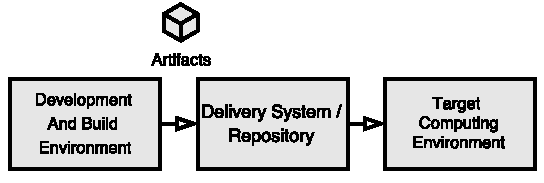
\includegraphics[width=.7\linewidth]{deployment_extended_process}
  \caption{Artifacts Deployment}
  \label{fig:deployment_extended_process}
\end{figure}

Deployment artifacts are the artifacts needed at the deployment environment. Artifacts are built at development and build environment. Built artifacts are move for a delivery system where they can be accessed from the target environment. At deployment the artifacts are moved from the delivery system to the target computing environment. Also, configuration activities can be realized.
In the software industry, a \emph{continuous integration}\cite{humble_continuous_2010} environment applies automation in building and getting components ready to delivery. In such environment if a developer pushes changes to a code repository, components are automatically built and published to delivery system. The build process commonly involves fetching build dependencies, compiling source code, running automated quality control (tests and static analysis) and packaging components into artifacts. Artifacts are published if target quality policies are met.
%dependency manager
Fundamental to continuous integration environments are \emph{Dependency Management Systems} tools, such as Maven\cite{apache_apache_2016} for Java platform. These tools simplify the management of software dependencies~\cite{spinellis_package_2012}. Such tools ensure that development team members are working with same dependencies that are used in the build environment.
%Sistemas de Gereencia de Pacotes simplificam o processo de instalacao de dependencias. Um pacote contem em um formato padronizado codigo ou codigo compilado, juntamente a sua documentacao e metadados [7]. Os metadados normalmente incluem nome, versao e especificacao de instalacao. Sistemas de Gerencia de Pacotes gerenciam a obtencao e instalac ̧a  ̃ o de dependˆ encias de forma automatizada, com o m ́ınimo de interac ̧ a  ̃o com o usu ́ ario e consequentemente favorecem a reprodutibilidade.
%build manager

Research in software configuration and deployment, has focused on responding to dynamisms in a known environment. This could be costs and failures in a cloud environmet \cite{ferreira_leite_user_2014}, changes in managed resources \citep{gunalp_rondo_2015}, and changes in the context of operation~\cite{bencomo_dynamically_2008}.

\emph{Continuous delivery}\cite{humble_continuous_2010} extends the continuous integration environment, moving components from the delivery system to a target computing environment with none or minimum human intervention.

In the industry, package managers such as aptitute/apt-get(Debian based Linux distributions) \cite{aoki_debian_2016}, yum (Red Hat based Linux distributions) \cite{svistunov_red_2016}, Homebrew (MacOS)\cite{homebrew_homebrew_2016} and Chocolatey (Windows)\cite{chocolatey_chocolatey_2016} are capable of solving dependencies and deploying software. They require that a managed application declare their dependencies by name and version. DevOps\cite{bang_grounded_2013} is a movement in software industry that advocates that all configuration steps needed to configure the computing environment should be written as code (\emph{infrastructure as code}), following best practices of software development. That movement favors the documentation, reproducibility, automation and scalability.
%Tools such as Puppet and Chef are used by devopers to manage infrastructure.
DevOps allows for management of scalable computing environments. It can offer a significant advantage for enterprise environment in relation to manual approaches in which system administrators configure the system by manually following configuration steps. Current continuous integration/delivery and DevOps practices are not sufficient for highly dynamic and heterogeneous target computing environments; they require that highly specialized system administrators to analyze the environment and create environment configuration descriptors.
%% Deployment in IoT??
